\documentclass[12pt]{article}
 
\usepackage[margin=1in]{geometry} 
\usepackage{amsmath,amsthm,amssymb, bm}
\usepackage{minted}
\usepackage{mdframed}
\usepackage{multicol}
\usepackage{graphicx}
\usepackage{parskip}

\newcommand{\N}{\mathbb{N}}
\newcommand{\Z}{\mathbb{Z}}
\newcommand{\haskell}{\mintinline{haskell}}

\newenvironment{lemma}[2][Lemma]{\begin{trivlist}
\item[\hskip \labelsep {\bfseries #1}\hskip \labelsep {\bfseries #2.}]}{\end{trivlist}}
\newenvironment{question}[2][Question]{\begin{trivlist}
\item[\hskip \labelsep {\bfseries #1}\hskip \labelsep {\bfseries #2.}]}{\end{trivlist}}
 
\begin{document}
 
\title{COM2001 Advanced Programming Topics}
\author{Assignment 2 - Theory} 
\date{}

\maketitle

%%%%%%%%%%%%%%%%%%%%%%%%%%%%% QUESTION 1 %%%%%%%%%%%%%%%%%%%%%%%%%%%%% 
\begin{question}{1}
\end{question}

\begin{lemma}{1}
Prove that \haskell{sLen (sPop (Append s x))} \haskell{==} 
\haskell{sLen s}
\end{lemma}

\begin{center}
Let $P(s) \equiv$ \haskell{sLen (sPop (Append s x))} \haskell{==} \haskell{sLen s}
\end{center}

\begin{proof}[\textbf{Lemma 1} Base Case]
$P(\haskell{None}) \equiv $ \haskell{sLen (sPop (Append None x))} \haskell{==} \haskell{sLen None}

\begin{mdframed}
\begin{minted}{haskell}
LHS: sLen (sPop (Append None x))
     = sLen (None)               -- [sPop.1]

RHS: sLen None
     == LHS
\end{minted}
\end{mdframed}
\end{proof}

\begin{proof}[\textbf{Lemma 1} Step Case]
Assume $P(s) \equiv$ \haskell{sLen (sPop (Append s x))} \haskell{==} 
\haskell{sLen s} is true. Prove $P(\haskell{Append s y})$, where 
\haskell{x} and \haskell{y} can be any values of same type.
\begin{mdframed}
\begin{minted}{haskell}
LHS: sLen (sPop (Append (Append s y) x))
     = sLen (Append (sPop (Append s y)) x) -- [sPop.n]
     = Succ (sLen (sPop (Append s y)))     -- [sLen.n]
\end{minted}     

according to assumption, \haskell{sLen (sPop (Append s x))} 
\haskell{==} \haskell{sLen s}
\begin{minted}{haskell}
     = Succ (sLen s)                       -- assumption
   
RHS: sLen (Append s y)
     = Succ (sLen s)
     == LHS
\end{minted}
\end{mdframed}
\end{proof}

\noindent To prove that \haskell{sLen str} \haskell{==} 
\haskell{sLen (sRev str)}, first
\begin{center}
Let $P(str) \equiv$ \haskell{sLen str} \haskell{==} \haskell{sLen (sRev str)}
\end{center}
and then, it is required to prove that $P(\haskell{None})$, $P(\haskell{s})$ and $P(\haskell{Append s x})$ holds whenever \haskell{s} is a finite length of type \haskell{Stream a}.

\newpage
\begin{proof}[Base Case]
When \haskell{str} is \haskell{None}
\begin{mdframed}
\begin{minted}{haskell}
LHS: sLen str 
     = sLen None
     = Zero             -- by [sLen.0]

RHS: sLen (sRev str) 
     = sLen (sRev None)
     = sLen (None)      -- by [sRev.0]
     = Zero             -- by [sLen.0]
     == LHS
\end{minted}
\end{mdframed}
Hence, the statement $P(\haskell{None})$ holds
\bigskip
\end{proof}

\begin{proof}[Step Case]
Assume that the statement $P(s) \equiv$ \haskell{sLen s} \haskell{==} 
\haskell{sLen (sRev s)} holds. Prove that the statement $P(\haskell{Append s y})$, 
where \haskell{y} can be any values of type \haskell{a}, also holds.

\begin{mdframed}
\begin{minted}{haskell}
LHS: sLen (Append s y) 
     = Succ (sLen s)                              -- by [sLen.n]
\end{minted}

according to \textbf{Lemma 1}, \haskell{sLen (sPop (Append s x))} 
\haskell{==} \haskell{sLen s}, hence
\begin{minted}{haskell}
     = Succ (sLen (sPop (Append s x)))            -- Lemma 1
     
RHS: sLen (sRev (Append s y))
     = sLen (Append (sRev s') y')                 -- [sRev.n]
\end{minted}

\begin{minted}{haskell}
  where  s' = sPop (Append s y)
         y' = sTop (Append s y)

     = Succ (sLen (sRev (sPop (Append s y)))      -- [sLen.n]
\end{minted}

Since \haskell{x} and \haskell{y} can be any values of the same type, and
the output of the function \haskell{sPop} is type \haskell{Stream a}. According
to our assumption, \haskell{sLen s} \haskell{==} \haskell{sLen (sRev s)}. Therefore, the statement \haskell{sLen (sPop (Append s x))} \haskell{==} 
\haskell{sLen (sRev (sPop (Append s y))} should be true even if \haskell{x} does not equal to \haskell{y} because the length of the stream is not affected by the value of 
\haskell{x} or \haskell{y}. Hence, \haskell{LHS == RHS}
\end{mdframed}
\end{proof}
According to the proofs above, it can be said that the statement $P(str) \equiv$ \haskell{sLen str} \haskell{==} \haskell{sLen (sRev str)} holds for all the finite defined values of
\haskell{str}, providing that the result produced can be represented by a value in the set of finite defined values of \haskell{Nat}.


%%%%%%%%%%%%%%%%%%%%%%%%%%%%% QUESTION 2 %%%%%%%%%%%%%%%%%%%%%%%%%%%%% 
\newpage\begin{question}{2}
\end{question}

\begin{proof}
Given three functions, as defined below:

\begin{enumerate}
\item \haskell{f :: Num a => Either Bool a -> b}
\item \haskell{g :: c -> Either c Int}
\item \haskell{h = \x -> x f g}
\end{enumerate}

\par\noindent The function \haskell{h} can be rewritten as
\begin{center}
\haskell{h x = x f g}
\end{center}
\textbf{Lemma 2.} \haskell{h} is a function which takes a function \haskell{x} as argument, and return the result of the function \haskell{x} taking two functions \haskell{f} and \haskell{g} as argument.

\begin{mdframed}
\flushleft \textbf{Step 1.} Assume \haskell{x :: a} \\
\noindent By Type Instantiation, \\
{\centering
    \begin{tabular}{cll}
    \haskell{x ::} & \haskell{a}                   & \\
    \haskell{x ::} & \haskell{a {d -> e -> t / a}} & \haskell{-- type instantiation} \\
    \haskell{x ::} & \haskell{d -> e -> t}         &
    \end{tabular}
\par}

\flushleft\par\noindent \textbf{Step 2.} Assume \haskell{f :: d}, where \haskell{d :: Num a => Either Bool a -> b} \\
\noindent By Function Application, \\
{\centering
    \begin{tabular}{cllclll}
    \haskell{ x  ::} & \haskell{d} & \haskell{->} & \haskell{e} & \haskell{->} & \haskell{t} & \\
    \haskell{ f  ::} & \haskell{d} &              &             &              &             & \haskell{-- assumed} \\ \cline{1-6}
    \haskell{x f ::} & \haskell{e} & \haskell{->} & \haskell{t} &              &             & \haskell{-- function application}
    \end{tabular}
\par}

\flushleft\par\noindent \textbf{Step 3.} Assume \haskell{g :: e}, where \haskell{e :: c -> Either c Int} \\
\noindent By Function Application, \\
{\centering
    \begin{tabular}{cllll}
    \haskell{ x f  ::} & \haskell{e} & \haskell{->} & \haskell{t} & \\
    \haskell{  g   ::} & \haskell{e} &              &             & \haskell{-- assumed} \\ \cline{1-4}
    \haskell{x f g ::} & \haskell{t} &              &             & \haskell{-- function application}
    \end{tabular}
\par}
\bigskip

\flushleft\par\noindent Since \haskell{h x = x f g}, hence the type of the function \haskell{h} should be \\
{\centering
    \haskell{h :: (d -> e -> t) -> t}.
\par}
\bigskip

But it is assumed that \haskell{d :: Num a => Either Bool a -> b}, substituting \haskell{d} back to \haskell{h}, \\
{\centering
    \haskell{h :: Num a => ((Either Bool a -> b) -> e -> t) -> t}
\par}
\bigskip

It is also assumed that \haskell{e :: c -> Either c Int}, substituting \haskell{e} back to \haskell{h}, \\
{\centering
    \haskell{h :: Num a => ((Either Bool a -> b) -> (c -> Either c Int) -> t) -> t}
\par}
\end{mdframed}
\end{proof}

To show that the proof above for the type of \haskell{h} is true, compare the result obtained above with the statement in \textbf{Lemma 2}.
\bigskip

In \textbf{Lemma 2}, it is stated that \haskell{h} takes a function \haskell{x} as argument, and return a result of type same as the result produced by the function \haskell{x} taking two arguments \haskell{f} and \haskell{g}.
\begin{mdframed}
Deduction:
\begin{enumerate}
    \item The type of the result of function \haskell{h} and function \haskell{x} should be the same, which in this case is \haskell{t}. This can be seen from the definition of function \haskell{h}, as the output of \haskell{h} is equal to \haskell{x f g}.
    \item According to \textbf{1}, then the type of \haskell{x f g} should be \haskell{t}.
    \item According to \textbf{2}, and since \haskell{x} takes \haskell{f} and \haskell{g} as arguments, and the  type of \haskell{x f g} is \haskell{t}, then the type of \haskell{x} should be \\
    \haskell{Num a => (Either Bool a -> b) -> (c -> Either c Int) -> t}
    \item According to the deductions above, it is known that the return type of \haskell{h} is \haskell{t}, and \haskell{h} only take function \haskell{x} as argument, therefore the type of the function \haskell{h} should be \\ \haskell{Num a => ((Either Bool a -> b) -> (c -> Either c Int) -> t) -> t}
\end{enumerate}
\end{mdframed}
The deductions above give the same result as the proof using the type inference rules. Therefore, it has been proved that the type of the function \haskell{h} is
\begin{center}
    \haskell{h :: Num a => ((Either Bool a -> b) -> (c -> Either c Int) -> t) -> t}
\end{center}


%%%%%%%%%%%%%%%%%%%%%%%%%%%%% QUESTION 3 %%%%%%%%%%%%%%%%%%%%%%%%%%%%% 
\newpage\begin{question}{3}
\end{question}

\begin{proof}
To prove that \haskell{diff} is a `totally correct' implementation of $\bm{\delta}$, it is required to prove that:
\begin{enumerate}
    \item \emph{Correctness}: For all finite defined lists, by giving \haskell{diff} and $\bm{\delta}$ the same input, \haskell{diff} should produced the same output as $\bm{\delta}$, and the output produced is the right answer.
    \item \emph{Total correctness}: The function \haskell{diff} will definitely halt.
\end{enumerate}

\begin{proof}[\textbf{1.} Proof of Correctness]
To prove the correctness of \haskell{diff}, let
\begin{center}
    $P(\haskell{xs}) \equiv$ \haskell{diff(xs, ys)} \haskell{==} $\bm{\delta}$(\haskell{xs, ys}), for all finite defined \haskell{ys} of type \haskell{[b]}
\end{center}

\begin{proof}[Base Case 1]
When $P(\haskell{[]}) \equiv$ \haskell{diff([], ys)} \haskell{==} $\bm{\delta}$(\haskell{[], ys}),
\begin{mdframed}
\begin{multicols}{2}
\begin{minted}{haskell}
LHS: diff([], ys)
    = - (length ys)
\end{minted}
\columnbreak
\haskell{RHS:} $ \bm{\delta}$(\haskell{[], ys}) \\
\haskell{    = -} $\bm{\delta}$(\haskell{ys, []}) \\
\haskell{    = - (length(ys) - length([]))} \\
\haskell{    = - length(ys)} \\
\haskell{    == LHS}
\end{multicols}
\end{mdframed}
\end{proof}

\begin{proof}[Step Case 1]
Assume that for all finite defined \haskell{ys} of type \haskell{[b]}, the statements
\begin{itemize}
    \item $P(\haskell{s}) \equiv$ \haskell{diff(s, ys)} \haskell{==} $\bm{\delta}$(\haskell{s, ys}) is true if \haskell{length s >= length ys}
    \item $P(\haskell{s}) \equiv$ \haskell{diff(s, ys)} \haskell{== -} $\bm{\delta}$(\haskell{ys, s}) is true if \haskell{length s < length ys}
\end{itemize}
When $P(\haskell{x:s}) \equiv$ \haskell{diff(x:s, ys)} \haskell{==} $\bm{\delta}$(\haskell{x:s, ys}) and \haskell{length x:s >= length ys}, 
\begin{mdframed}
\begin{minted}[escapeinside=||,mathescape=true]{haskell}
LHS: diff(x:s, ys)
  = diff(x ++ s, [] ++ ys)
  = diff(x, []) + diff(s, ys)
  = length x + diff(s, ys)                -- case definition
  = length x + |$ \bm{\delta}$|(s, ys)                   -- assumption

RHS: |$\bm{\delta}$|(x:s, ys)
    = length(x:s) - length(ys)            -- $\bm{\delta}$ definition
    = length(x) + length(s) - length(ys)
    = length(x) + |$\bm{\delta}$|(s, ys)                -- $\bm{\delta}$ definition
    == LHS
\end{minted}
\end{mdframed}

\newpage When $P(\haskell{x:s}) \equiv$ \haskell{diff(x:s, ys)} \haskell{== -} $\bm{\delta}$(\haskell{ys, x:s}) and \haskell{length x:s < length ys}, 
\begin{mdframed}
\begin{minted}[escapeinside=||,mathescape=true]{haskell}
LHS: diff(x:s, ys)
  = diff(x ++ s, [] ++ ys)
  = diff(x, []) + diff(s, ys)
  = length x + diff(s, ys)                  -- case definition
  = length x - |$ \bm{\delta}$|(ys, s)                     -- assumption

RHS: |$\bm{\delta}$|(x:s, ys)
    = - |$\bm{\delta}$|(ys, x:s)
    = - length(ys) + length(x:s)            -- $\bm{\delta}$ definition
    = - length(ys) + length(x) + length(s)
    = length(x) - length(ys) + length(s)
    = length(x) - |$\bm{\delta}$|(ys, s)                  -- $\bm{\delta}$ definition
    == LHS
\end{minted}
\end{mdframed}
\end{proof}
It has been proved that the statements $P(\haskell{[]})$, $P(\haskell{s})$, and $P(\haskell{x:s})$ are true for all finite defined \haskell{ys} of type \haskell{[b]}. Therefore, it can be stated that the statement
\begin{center}
    $P(\haskell{xs}) \equiv$ \haskell{diff(xs, ys)} \haskell{==} $\bm{\delta}$(\haskell{xs, ys}), for all finite defined \haskell{ys} of type \haskell{[b]}
\end{center}
is true as well.

\bigskip\bigskip\par\noindent Now, let
\begin{center}
    $P(\haskell{ys}) \equiv$ \haskell{diff(xs, ys)} \haskell{==} $\bm{\delta}$(\haskell{xs, ys}), for all finite defined \haskell{xs} of type \haskell{[a]}
\end{center}

\begin{proof}[Base Case 2]
When $P(\haskell{[]}) \equiv$ \haskell{diff(xs, [])} \haskell{==} $\bm{\delta}$(\haskell{xs, []}),
\begin{mdframed}
\begin{multicols}{2}
\begin{minted}{haskell}
LHS: diff(xs, [])
    = length xs
\end{minted}
\columnbreak
\haskell{RHS:} $ \bm{\delta}$(\haskell{xs, []}) \\
\haskell{    = length(xs) - length([])} \\
\haskell{    = length(xs)} \\
\haskell{    == LHS}
\end{multicols}
\end{mdframed}
\end{proof}

\begin{proof}[Step Case 2]
Assume that for all finite defined \haskell{xs} of type \haskell{[a]}, the statements
\begin{itemize}
    \item $P(\haskell{s}) \equiv$ \haskell{diff(xs, s)} \haskell{==} $\bm{\delta}$(\haskell{xs, s}) is true if \haskell{length xs >= length s}
    \item $P(\haskell{s}) \equiv$ \haskell{diff(xs, s)} \haskell{== -} $\bm{\delta}$(\haskell{s, xs}) is true if \haskell{length xs < length s}
\end{itemize}
 When $P(\haskell{y:s}) \equiv$ \haskell{diff(xs, y:s)} \haskell{==} $\bm{\delta}$(\haskell{xs, y:s}) and \haskell{length xs >= length y:s},
\begin{mdframed}
\begin{minted}[escapeinside=||,mathescape=true]{haskell}
LHS: diff(xs, y:s)
  = diff([] ++ xs, y ++ s)
  = diff([], y) + diff(xs, s)
  = - (length y) + diff(xs, s)              -- case definition
  = - (length y) + |$ \bm{\delta}$|(xs, s)                 -- assumption

RHS: |$\bm{\delta}$|(xs, y:s)
    = length(xs) - length(y:s)              -- $\bm{\delta}$ definition
    = length(xs) - (length(y) + length(s))
    = length(xs) - length(y) - length(s)
    = - length(y) + length(xs) - length(s)
    = - length(y) + |$\bm{\delta}$|(xs, s)                -- $\bm{\delta}$ definition
    == LHS
\end{minted}
\end{mdframed}

When $P(\haskell{y:s}) \equiv$ \haskell{diff(xs, y:s)} \haskell{== -} $\bm{\delta}$(\haskell{y:s, xs}) and \haskell{length xs < length s},
\begin{mdframed}
\begin{minted}[escapeinside=||,mathescape=true]{haskell}
LHS: diff(xs, y:s)
  = diff([] ++ xs, y ++ s)
  = diff([], y) + diff(xs, s)
  = - (length y) + diff(xs, s)               -- case definition
  = - (length y) - |$ \bm{\delta}$|(s, xs)                  -- assumption

RHS: |$\bm{\delta}$|(xs, y:s)
    = - |$\bm{\delta}$|(y:s, xs)                           -- $\bm{\delta}$ definition
    = - length(y:s) + length(xs)             -- $\bm{\delta}$ definition
    = - length(y) - length (s) + length(xs)
    = - length(y) - |$ \bm{\delta}$|(s, xs)                 -- $\bm{\delta}$ definition
    == LHS
\end{minted}
\end{mdframed}
\end{proof}
It has been proved that the statements $P(\haskell{[]})$, $P(\haskell{s})$, and $P(\haskell{y:s})$ are true for all finite defined \haskell{xs} of type \haskell{[a]}. Therefore, it can be stated that the statement
\begin{center}
    $P(\haskell{ys}) \equiv$ \haskell{diff(xs, ys)} \haskell{==} $\bm{\delta}$(\haskell{xs, ys}), for all finite defined \haskell{xs} of type \haskell{[a]}
\end{center}
is true as well.

\noindent Since it has been proved that 
\begin{enumerate}
    \item For all finite defined \haskell{ys} of type \haskell{[b]}, $P(\haskell{xs})$ is true
    \item For all finite defined \haskell{xs} of type \haskell{[a]}, $P(\haskell{ys})$ is true
\end{enumerate}
Hence, the \emph{correctness} of \haskell{diff} has been proved, and \haskell{diff} is a correct implementation of the function $\bm{\delta}$.
\end{proof}

\newpage\begin{proof}[\textbf{2.} Proof of Total Correctness]
The \emph{correctness} of \haskell{diff} has been proved. To prove that \haskell{diff} is a totally correct implementation of $\bm{\delta}$, it is required to show that \haskell{diff} is correct, and \haskell{diff} will definitely halt.
\begin{mdframed}
  \begin{center}
    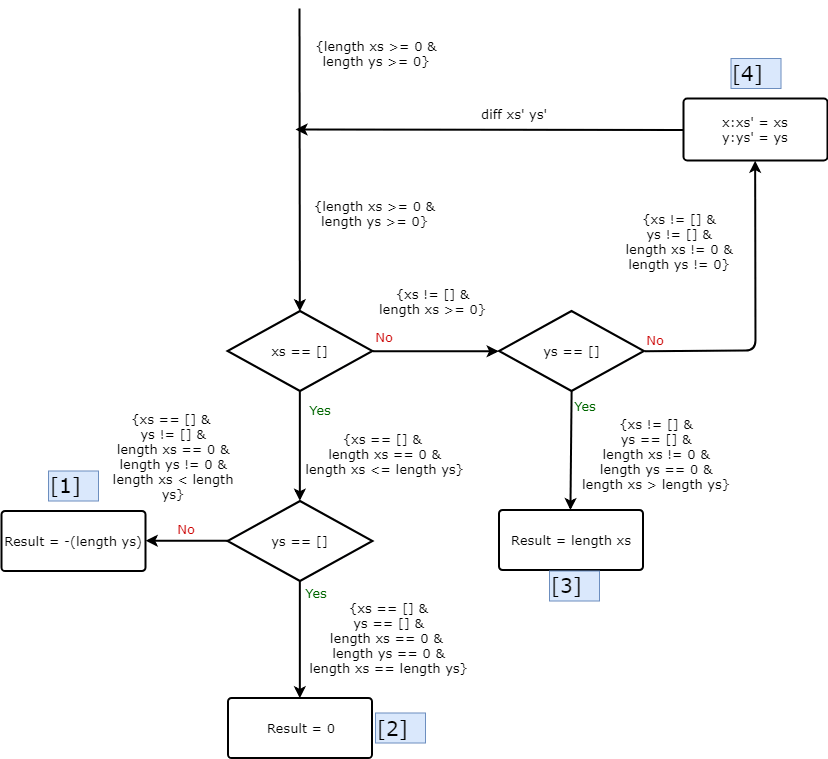
\includegraphics[width=15.7cm]{flowchart.png}
    \textbf{Figure 1. Flowchart (Floyd-Hoare Logic) of} \haskell{diff} \textbf{function}
  \end{center}
\end{mdframed}

\textbf{Figure 1} showed the flowchart of function \haskell{diff} drawn according to Floyd-Hoare Logic. To show that \haskell{diff} will definitely halt, four cases are considered.

\par\noindent \textbf{Case [1]:} \emph{Base case}. This is when \haskell{xs} is \haskell{[]} and \haskell{ys} is some finite defined list. In this case, the function \haskell{diff} will always halt because the pattern \haskell{([], ys)} is defined in the  case expressions of \haskell{diff}, and the result is \haskell{- (length ys)}. Therefore, \haskell{diff} will directly return the result whenever the pattern is matched.

\bigskip\par\noindent \textbf{Case [2]:} \emph{Base case}. This is when both \haskell{xs} and \haskell{ys} are \haskell{[]}. The pattern \haskell{([], [])} is defined in the case expressions of \haskell{diff} as well, and the result is \haskell{0}. Hence, \haskell{diff} will halt when \haskell{xs} and \haskell{ys} are \haskell{[]}.

\bigskip\par\noindent \textbf{Case [3]:} \emph{Base case}. This is the opposite case of \textbf{Case [1]}, where \haskell{xs} is some finite defined list, and \haskell{ys} is \haskell{[]}. For this case, \haskell{diff} will halt as well because the pattern \haskell{(xs, [])} is also defined in the case expressions of \haskell{diff}, and the result is \haskell{length xs}.

\bigskip\par\noindent \textbf{Case [4]:} \emph{Recursive case}. When none of the patterns in \textbf{Case [1]}, \textbf{Case [2]}, and \textbf{Case [3]} are matched, then the function \haskell{diff} will call itself with arguments \haskell{xs'} and \haskell{ys'}, as shown in \textbf{Figure 1} above, where
\begin{itemize}
    \item \haskell{xs'} is defined as the tail of the original list \haskell{xs} (\haskell{x:xs' = xs})
    \item \haskell{ys'} is defined as the tail of the orignal list \haskell{ys} (\haskell{y:ys' = ys})
\end{itemize}
For every recursion call, the function \haskell{diff} will be taking \haskell{xs'} as the new \haskell{xs}, and \haskell{ys'} as the new \haskell{ys}. Since \haskell{xs'} and \haskell{ys'} are the tail of their original list, therefore, \haskell{xs'} and \haskell{ys'} are one length shorter than their previous list. The recursion stops when the pattern of the `new' \haskell{(xs, ys)} is matched with one of the \emph{Base case}.

Now it is required to show that the \emph{recursive case} of \haskell{diff} will eventually halt. It is known that
\begin{enumerate}
    \item \textbf{Condition 1:} The \haskell{length} of a list cannot be less than \haskell{0}
    \item \textbf{Condition 2:} \haskell{xs} and \haskell{ys} are some finite defined lists
\end{enumerate}
The recursion terminates when it is one of the case:
\begin{enumerate}
    \item \textbf{Case [1]:} \haskell{diff([], ys)}, which means \haskell{length xs < length ys}
    \item \textbf{Case [2]:} \haskell{diff([], [])}, which means \haskell{length xs = length ys}
    \item \textbf{Case [3]:} \haskell{diff(xs, [])}, which means \haskell{length xs > length ys}
\end{enumerate}
Since the recursive step of \haskell{diff} is just removing the head of both lists, and \textbf{Condition 1} and \textbf{Condition 2} must be satisfied. After finite amount of recursion step, eventually one or both of the lists will become empty. As a result, it must be \textbf{Case [1]}, \textbf{Case [2]} or \textbf{Case [3]} which causes the recursion to terminates. Therefore, it has been proved that the function \haskell{diff} will definitely halt. \\
\end{proof}

It has been proved that
\begin{enumerate}
    \item \emph{Correctness}: For all finite defined lists, by giving \haskell{diff} and $\bm{\delta}$ the same input, \haskell{diff} should produced the same output as $\bm{\delta}$, and the output produced is the right answer.
    \item \emph{Total correctness}: The function \haskell{diff} will definitely halt.
\end{enumerate}
Hence, the function \haskell{diff} is a totally correct implementation of the function $\bm{\delta}$. \\
\end{proof}


% %%%%%%%%%%%%%%%%%%%%%%%%%%%%% QUESTION 4 %%%%%%%%%%%%%%%%%%%%%%%%%%%%% 
\newpage\begin{question}{4}
\end{question}

Since the function \haskell{sRev} involves calling other two function, \haskell{sPop} and \haskell{sTop}. Therefore, it is required to convert \haskell{sPop} to \haskell{sPopT} and \haskell{sTop} to \haskell{sTopT} where the result of their type is \haskell{Int}. It is also required to convert \haskell{sLen} to \haskell{sLenT} to return the result in type \haskell{Int} instead of \haskell{Nat}.

In the conversions below, since \haskell{Append} is a data type, it is assumed that \haskell{Append} has no cost.

Converting \haskell{sLen} into \haskell{sLenT},
\begin{mdframed}
\begin{minted}{haskell}
sLenT :: Stream a -> Int
sLenT s = case s of
  None         -> 0
  Append s' _  -> 1 + (sLenT s')
\end{minted}
\end{mdframed}

Converting \haskell{sPop} into \haskell{sPopT},
\begin{mdframed}
\begin{minted}[escapeinside=||,mathescape=true]{haskell}
|$T_{sPop}$| None = 1 + T(None) -- cost:case
|\hspace{2.23cm}|= 1 + 0       -- cost:var
|\hspace{2.23cm}|= 1           -- arithmetic

|$T_{sPop}$| Append None _  = 1 + T(None)  -- cost:case
|\hspace{4.4cm}|= 1 + 0        -- cost:var
|\hspace{4.4cm}|= 1            -- arithmetic

|$T_{sPop}$| Append s' x  = 1 + T(Append (sPop s') x)         -- cost:case
|\hspace{3.97cm}|= 1 + T(Append) + T(sPop s') + T(x) -- cost:func
|\hspace{3.97cm}|= 1 + 0 + T(sPop s') + 0            -- cost:const
|\hspace{3.97cm}|= 1 + 0 + |$T_{sPop}$| s' + 0 |\hspace{2.98cm}|-- cost:func
|\hspace{3.97cm}|= 1 + T(sPop s')                    -- arithmetic
|\hspace{3.97cm}|= 1 + |$T_{sPop}$| s' |\hspace{4.72cm}|-- cost:func
|\hspace{3.97cm}|= 1 + sPopT s'                -- substitution of sPopT
|\hspace{3.97cm}|= 1 + sLenT s' + 1            -- substitution of sLenT
|\hspace{3.97cm}|= 2 + sLenT s'                -- arithmetic
\end{minted}
Since \haskell{sPop} is a recursive function, where it loops all the way to the first \\ \haskell{Append (Stream a) a} and remove it. Therefore, \haskell{sPopT s'} equals to \haskell{sLenT s' + 1}, where the 1 is for the \haskell{sPopT None} case because \haskell{sLenT None} returns \haskell{0}.

\begin{minted}[escapeinside=||,mathescape=true]{haskell}
sPopT :: Stream a -> Int
sPopT s = case s of
  None           -> 1             -- $T_{sPop}$ None  
  Append None _  -> 1             -- $T_{sPop}$ Append None _
  Append s' x    -> 2 + sLenT s'  -- $T_{sPop}$ Append s' x
\end{minted}
\end{mdframed}

Converting \haskell{sTop} into \haskell{sTopT},
\begin{mdframed}
\begin{minted}[escapeinside=||,mathescape=true]{haskell}
|$T_{sTop}$| None = 1 + T(special) -- cost:case
|\hspace{2.23cm}|= 1 + 0          -- cost:var
|\hspace{2.23cm}|= 1              -- arithmetic

|$T_{sTop}$| Append None x = 1 + T(x)  -- cost:case
|\hspace{4.17cm}|= 1 + 0     -- cost:var
|\hspace{4.17cm}|= 1         -- arithmetic

|$T_{sTop}$| Append s' _  = 1 + T(sTop s')   -- cost:case
|\hspace{3.97cm}|= 1 + |$T_{sTop}$| s' |\hspace{1.03cm}|-- cost:func
|\hspace{3.97cm}|= 1 + sTopT s'     -- substitution of sTopT
|\hspace{3.97cm}|= 1 + sLenT s' + 1
|\hspace{3.97cm}|= 2 + sLenT s'     -- arithmetic
\end{minted}

\par\noindent \haskell{sTop} is a recursive function similar to \haskell{sPop}, where it loops all the way to the first \haskell{Append (Stream a) a} and returns the \haskell{a}. Hence, \haskell{sTopT s'} is equal to \haskell{sLenT s' + 1} too.

\begin{minted}[escapeinside=||,mathescape=true]{haskell}
sTopT :: Distinguished a => Stream a -> Int
sTopT s = case s of
  None           -> 1             -- $T_{sTop}$ None  
  Append None _  -> 1             -- $T_{sTop}$ Append None s
  Append s' _    -> 2 + sLenT s'  -- $T_{sTop}$ Append s' _
\end{minted}
\end{mdframed}

Converting \haskell{sRev} into \haskell{sRevT},
\begin{mdframed}
\begin{minted}[escapeinside=||,mathescape=true]{haskell}
|$T_{sRev}$| None = 1 + T(None) -- cost:case
|\hspace{2.23cm}|= 1 + 0       -- cost:var
|\hspace{2.23cm}|= 1           -- arithmetic

|$T_{sRev}$| Append None _ = 1 + T(s)  -- cost:case
|\hspace{4.17cm}|= 1 + 0     -- cost:var
|\hspace{4.17cm}|= 1         -- arithmetic

|$T_{sRev}$| _  = 1 + T(Append (sRev (sPop s)) (sTop s))        -- cost:case
|\hspace{1.79cm}|= 1 + T(Append) + T(sRev (sPop s)) + T(sTop s)  -- cost:func
|\hspace{1.79cm}|= 1 + 0 + T(sRev (sPop s)) + T(sTop s)          -- cost:const
|\hspace{1.79cm}|= 1 + 0 + |$T_{sRev}$| (sPop s) + T(sPop s) + T(sTop s) -- cost:func
|\hspace{1.79cm}|= 1 + 0 + |$T_{sRev}$| (sPop s) + |$T_{sPop}$| s + |$T_{sTop}$| s |\hspace{1.19cm}|-- cost:func
|\hspace{1.79cm}|= 1 + 0 + sRevT (sPop s) + sPopT s + sTopT s    -- cost:func
|\hspace{1.79cm}|= 1 + 0 + sRevT (sPop s) + (2 + sLenT s') + (2 + sLenT s') -- sub.
|\hspace{1.79cm}|= 5 + (2 * sLenT s') + sRevT (sPop s)            -- arithmetic



sRevT :: Distinguished a => Stream a -> Int
sRevT s = case s of
  None           -> 1
  Append None _  -> 1
  _              -> 5 + (2 * sLenT s') + sRevT (sPop s)
\end{minted}
\end{mdframed}

The main input is \haskell{Stream a}, so the most sensible `\textbf{size}' parameter for the cost function is the length of the given \haskell{Stream a}.

\bigskip Finding the cost function of \haskell{sRev},
\begin{mdframed}

\begin{minted}[escapeinside=||,mathescape=true]{haskell}
|From| |$T_{sRev}$| None = 1, 
|hence| |$C_{sRev}$| (0) = 1

|From| |$T_{sRev}$| Append None _ = 1, 
|hence| |$C_{sRev}$| (0) = 1

|From| |$T_{sRev}$| _ = 3 + (2 * sLenT s') + sRevT (sPop s),
|hence| |$C_{sRev}$| (n+1) = 3 + (2 * n) + |$C_{sRev}$| (n)
\end{minted}

\bigskip By recurrence rules,
\begin{minted}[escapeinside=||,mathescape=true]{haskell}
f(0) = d
f(n) = f(n-1) + b * n + c
\end{minted}

\bigskip Converting $C_{sRev}$ into closed form, 
\begin{minted}[escapeinside=||,mathescape=true]{haskell}
|$C_{sRev}$| (0) = 1
|$C_{sRev}$| (n+1) = 5 + (2 * n) + |$C_{sRev}$| (n)

|$C_{sRev}$| (n) = 5 + (2 * (n-1)) + |$C_{sRev}$| (n-1)
|\hspace{2.07cm}|= |$C_{sRev}$| (n-1) + (2 * n) + 3

\end{minted}
Substituting the values of $\bm{d = 1}$, $\bm{b = 2}$, $\bm{c = 3}$ into $f(n) = \cfrac{b}{2}\,n^{2} + (c + \cfrac{b}{2}\,)\,n + d$,
\newpage\par\noindent So the cost function of \haskell{sRev} is
\setlength{\abovedisplayskip}{0pt}
\begin{align*}
C_{sRev} (n) &= \cfrac{2}{2}\,n^{2} + (3 + \cfrac{2}{2}\,)\,n + 1 \\
&= n^{2} + 4n + 1
\end{align*}
Therefore, \haskell{sRev} is tractable, and its worst-case complexity class is $\bm{O(n^{2}})$.
\end{mdframed}

\end{document}
